%*******************************************************************************
%****************************** Second Chapter *********************************
%*******************************************************************************

\chapter{The Model and Simulation Methods}
\graphicspath{{Chapter2/Figs/}}

To model the chromosome movements during nuclear osculation in fission yeast, let us start from a single chromosome modeled by a single polymer loop. 
In this chapter, we will introduce the details of the polymer model for the chromosomes and the simulation methods that resolving the dynamics and statistics of the polymer. 


%********************************** %First Section  **************************************
\section{The pulled polymer loop model}
\label{sec:the_pulled_polymer_loop_model}

As mentioned in the previous chapter, there are three pairs of chromosomes in fission yeast. During nuclear oscillation, these three pairs of chromosomes bound to one point, i.e. the Spindle Pole Body (SPB). Now let us start from the simplest case and neglect the interactions between chromosomes, think about a single chromosome. It is a polymer with ring structure, and an external force is exerted on the SPB. We have two choices to model this chromosome, i.e. the bead-rod model or the bead-spring model. We will use both models in this thesis but more discussions are focused on the bead-rod. Both models have their own benefits and shortcomings. Computationally, it is easier to manipulate the bead-spring model than the bead-rod. However, the bead-rod has the intrinsic property of finite extensible without resorting to some complex nonlinear spring potentials. This benefit we think is important because the chromosomes are highly condensed and are definitely finite extensible. In fact, we will show that the finite extensibility takes an important role for the polymer dynamics, see in the later chapters. And the simplicity of bead-rod model offers us the possibility to find analytical solutions. 

In this section, we will introduce both the bead-rod and bead-spring model for modeling the chromosomes. However, before that, let us first do a coordinate transformation that makes our analysis much easier. 

\subsection{Coordinate transformation}
\label{sub:coordinate_transformation}
Let us consider a single chromosome pulled at the SPB. The pulling force drives the chromosome moves with a velocity $\mathbf{v}$. In our model, the SPB is modeled as one monomer of the polymer loop. Other monomers representing the chromosome move together with the SPB because of the bonds. This scenario of pulled polymer loop is shown in Fig. \ref{fig:coordinate} (a). 
\begin{figure}[htpb]
    \centering
    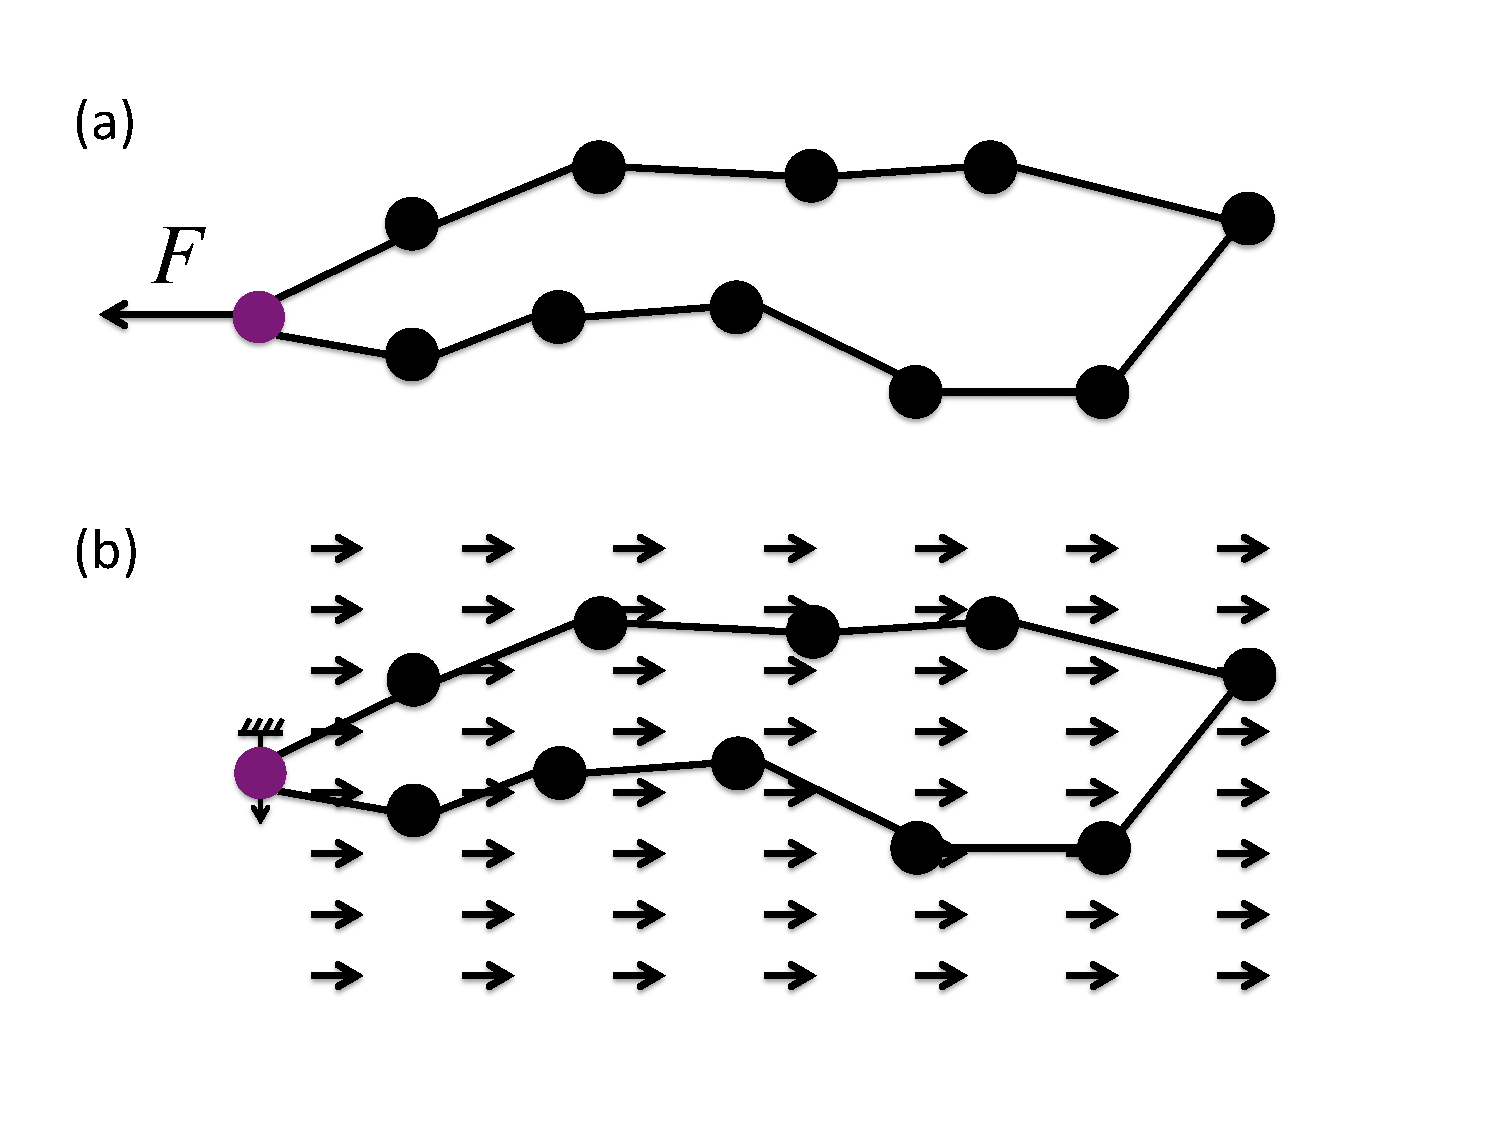
\includegraphics[width=0.8\linewidth]{coordinate}
    \caption{Illustration of coordinate transformation. (a) a pulled polymer loop before transformation; (b) pinned polymer loop in an external field after transformation. }
    \label{fig:coordinate}
\end{figure}

Now let us image we are sitting on the SPB. Then effectively, the SPB is pinned, and the polymer loop is immersed in a flow with velocity $-\mathbf{v}$, see in Fig. \ref{fig:coordinate} (b). Let us assume the Stoke's law is valid and according to that, there is a force $\mathbf{F}^e = - \xi \mathbf{v}$ exerting on every bead. $\xi$ is the friction coefficient for the bead in the solution.

In conclusion, the pulled polymer loop model is equivalent to the pinned polymer loop in an external force field. In our analysis, we will use the pinned polymer loop picture, because it is more easily to deal with both numerically and analytically. 


\subsection{The bead-rod model}
\label{sub:the_bead_rod_model}
Now let us come to a concrete polymer model for modeling the chromosomes, i.e. the bead-rod model. For this model, the beads representing chromosome segments are connected by massless rigid rod. For simplicity, we assume the length of every rod is identical, denote by $a$. The rigidity of the rod means the distance between two neighboring beads is fixed. 
\begin{figure}[htpb]
    \centering
    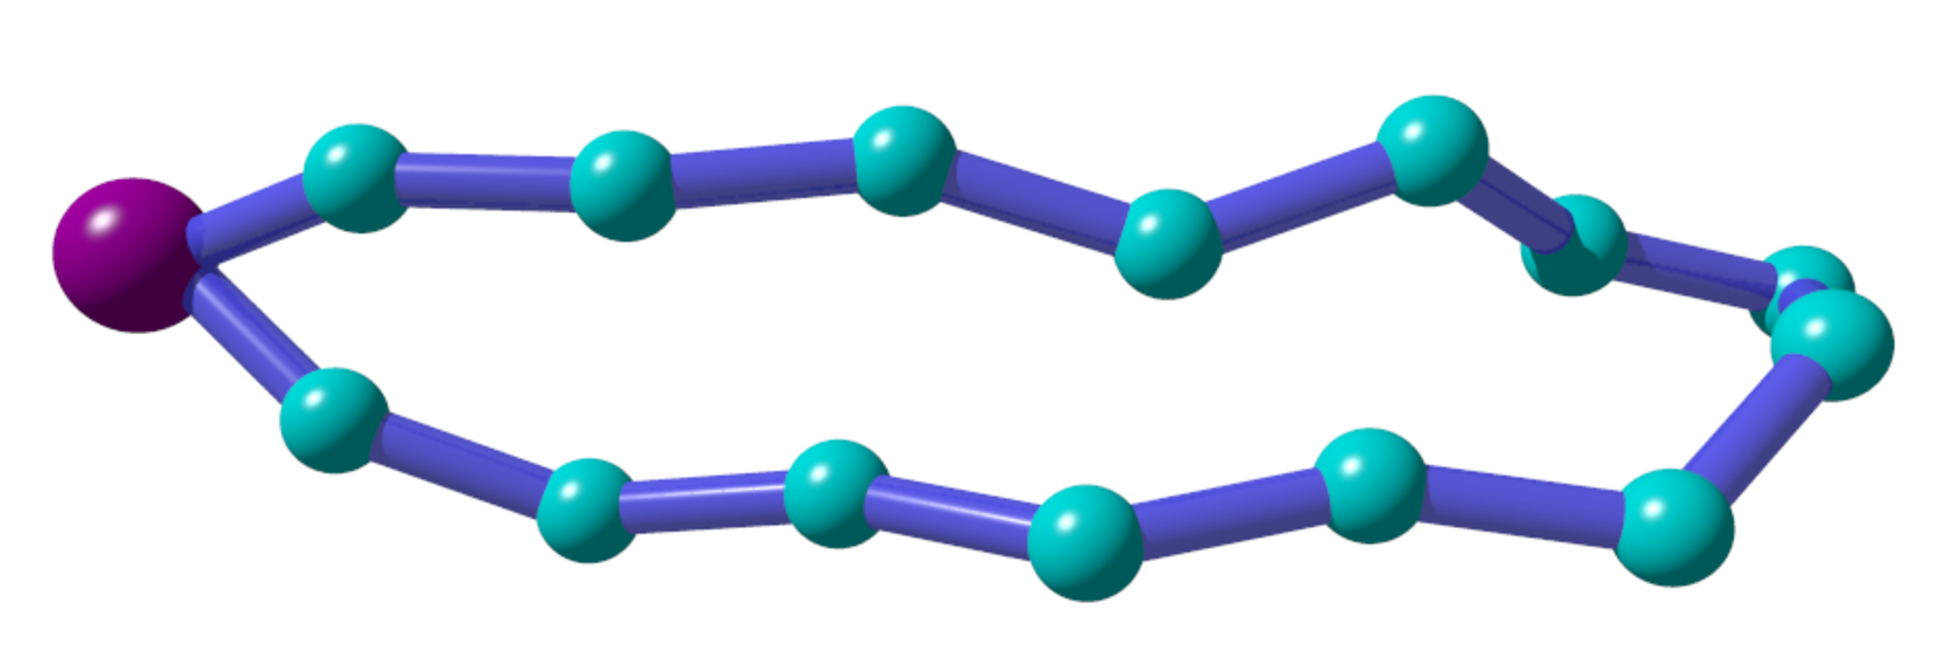
\includegraphics[width=0.8\linewidth]{beadrod}
    \caption{Sketch of the bead-rod loop model. The magenta bead represents the SPB and other cyan beads represent the chromosome segments.}
    \label{fig:beadrod}
\end{figure}

The dynamics of the polymer is specified by the motion of the beads. We shall first give out the dynamical equation and then explain how does it come from. Let say the contour length of the polymer loop is $L$, i.e. there are $L$ beads (including the SPB) and $L$ rods in the polymer. Denote the beads by the index $i = 0, 1, 2\cdot , L-1$, then the dynamical equation of $i^{\rm {th}}$ bead can be written as
\begin{equation}
    \label{eq:beadrodEq}
    \xi \frac{d \mathbf{r}_i}{d t} = \mathbf{F}_i^{u} + \mathbf{F}_i^{c} + \mathbf{F}_i^{pseudo} + \mathbf{F}_i^{e} + \mathbf{F}_i^{b}
\end{equation}
where $\xi$ is the friction coefficient of the bead in the solution, $\mathbf{F}_i^{u}$ is the interaction force specified by some kind of potentials, $\mathbf{F}_i^{c}$ is the constraint force that keeps the rod length fixed, $\mathbf{F}_i^{e}$ is the external force and $\mathbf{F}_i^{b}$ is the Brownian force caused by thermal fluctuations. And what is left in the right hand of Eq. \eqref{eq:beadrodEq} is $\mathbf{F}_i^{pseudo}$, which is a special type of force introduced in the bead-rod model in order to get the correct statistics. We will discuss more about it later. 

Now let us come back to explain how does Eq. \eqref{eq:beadrodEq} come from.  Firstly, notice that $\mathbf{F}_i^b$ in the equation is a stochastic variable, so Eq. \eqref{eq:beadrodEq} is actually a stochastic differential equation. Secondly, the left hand side of Eq. \eqref{eq:beadrodEq} is actually rearranged from the friction force of the bead in the solution $-\xi\mathbf{v}_i$. And we have assumed the solution is homogeneous so that the friction coefficient is independent of the space and time. Third, the inertial of the bead is neglected due to millions of collisions per second from the water molecules. In other word, Eq. \eqref{eq:beadrodEq} essentially can be written as $\mathbf{F}_i^{total} = \mathbf{0}$. This is simply the Newton's law with inertial neglected. This kind of dynamics of commonly used in polymer physics and called Brownian Dynamics \cite{}. 

Let us now discuss each term of the right hand side of Eq. \eqref{eq:beadrodEq} one by one. 

$\bullet$ Brownian force $\mathbf{F}_i^{b}$

The Brownian force can be caused by the enormous instantaneous collisions of the solvent molecules or by other sort of interactions between chromosomes and proteins in the nucleus. The level of fluctuation can be characterized by an effective temperature $T$. Mathematically, the Brownian force is described by a Gaussian process with the zero mean in space and time and the non-zero second moment, which can be written as:
\begin{subequations}
    \label{eq:brownianforce}
    \begin{equation}
        \left<\mathbf{F}_i^b\right> =\mathbf{0} 
    \end{equation}
    \begin{equation}
        \left<\mathbf{F}_i^b(t)\mathbf{F}_j^b(t^{\prime})\right> = 2k_B T \xi \delta_{ij} \delta(t-t^{\prime})
    \end{equation}
\end{subequations}
here, $\xi$ is the friction coefficient. $k_B$ is the Boltzmann constant. $\delta_{ij}$ is the Kronecker delta means there is no correlation for the Brownian force exerting on different beads. The second $\delta$ is the Dirac delta function. 

$\bullet$ External force $\mathbf{F}_i^{e}$

The external force in our pinned polymer loop model is simply the equivalent flow field after coordinate transformation. So we have $\mathbf{F}_i^e = \xi \mathbf{v}_{\rm{SPB}}$. In general, $\mathbf{v}_{\rm{SPB}} = \mathbf{v}_{\rm{SPB}}(t)$ is a function of time. However, when we consider the simplest case that the chromosome is pulled to move steadily in one direction, $\mathbf{v}_{\rm{SPB}}$ is a constant.

$\bullet$ Constraint force $\mathbf{F}_i^{c}$

The constraint force is the tension force on the rod to keep the length fixed. So the direction of the force is along the rod orientation. The rigid rod constraint can be written as 
\begin{equation}
    \label{eq:rodConstraint}
    |\mathbf{r}_{i+1} - \mathbf{r}_i| - a = 0
\end{equation}
where periodic index is utilized, i.e. $\mathbf{r}_{L} = \mathbf{r}_0$. The constraint force is an implicit force that depends on the other force exerting on the beads. We will discuss how to calculate this force in next section. 

$\bullet$ \emph{Pseudo} force $\mathbf{F}_i^{pseudo}$

The \emph{Pseudo} force is special virtual force that added in order to obtain the statistics we want. If we neglect the bending energy, excluded volume effect and other complex interactions in the model, we are essentially talking about the simplest freely joint polymer model. For such a simple model, we expect the random walk statistics, i.e. the orientation of two consecutive rods is independent. So the distribution of the included angle of two rods should be uniform. However, we cannot obtain this statistics as we want without the \emph{pseudo} force.

Let us take a simple example, the distribution of included angle of a trimer in 3D. Denote the angle as $\theta$. The 3D spherical uniform distribution can be written as
\begin{equation}
    \label{eq:trimerUniform}
    p(\theta) = const. \sin\theta
\end{equation}
On the other hand, the distribution of rigid bead-rod trimer without \emph{pseudo} force can be derived using the generalized coordinate
\begin{equation}
    \label{eq:trimerRigid}
    p(\theta) = const. (1-\frac{1}{4}\cos^2\theta)^{1/2}\sin\theta
\end{equation}
So they are not the same as we see here. The reason for this discrepancy is the rigidity of constraints reduce the phase space of the trimer from $6$ dimensional gully to $4$ dimension manifold. The simple Brownian force ensures the probability is uniform among the manifold but not $\theta$. 
\begin{figure}[htpb]
    \centering
    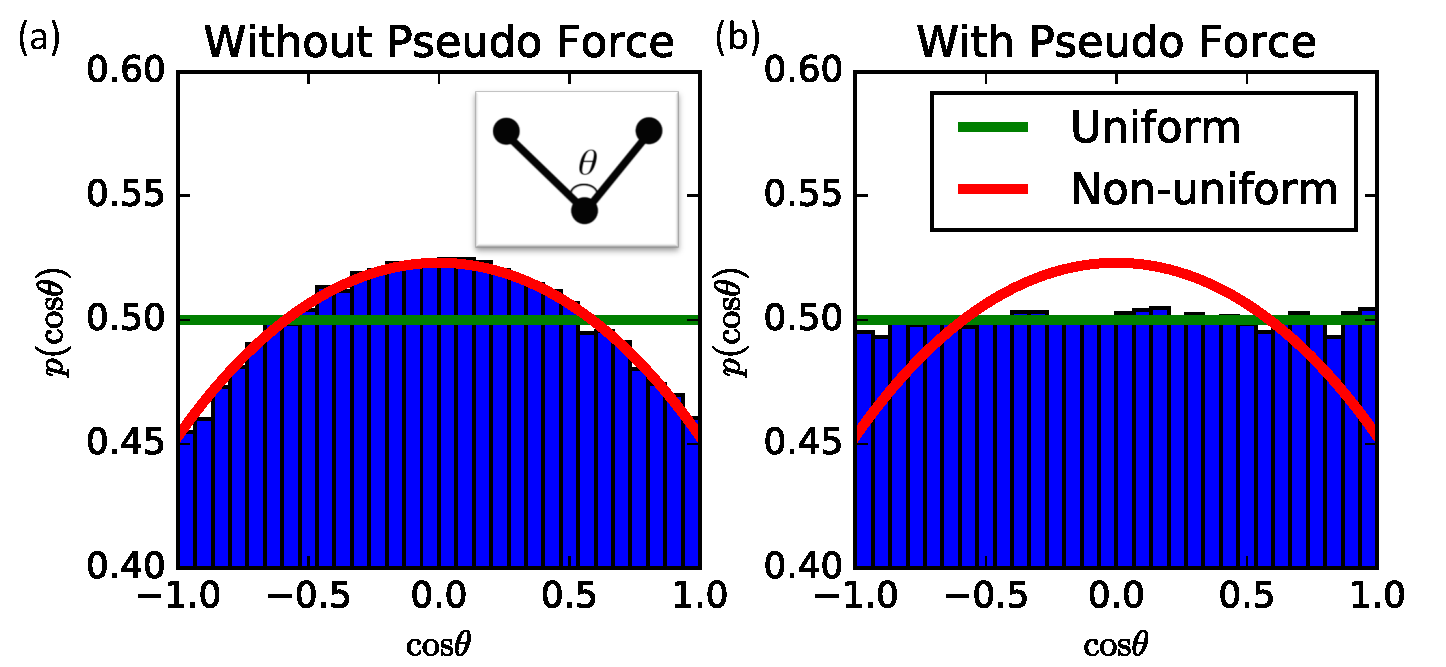
\includegraphics[width=1.0\linewidth]{trimer}
    \caption{The distribution of included angle of a bead-rod trimer. (a) without \emph{pseudo} force; (b) with \emph{pseudo} force. The blue bins are from Brownian Dynamics simulation results. Inset of (a) is a sketch for the trimer. }
    \label{fig:trimer}
\end{figure}

To solve the problem and obtain the statistics we want, Fixman introduced an effective \emph{pseudo} potential depends on the polymer configuration \cite{Fixman1974}, and hence we have a \emph{pseudo} force in Eq. \eqref{eq:beadrodEq}. The explicit form of the \emph{pseudo} force can be written as
\begin{subequations}
    \label{eq:pseudoForce}
    \begin{equation}
        \mathbf{F}_i^{pseudo} = -\frac{\partial U_{met}}{\partial\mathbf{r}_i}
    \end{equation}
    \begin{equation}
        U_{met} = \frac{1}{2}k_B T \ln(\det G)
    \end{equation}
\end{subequations}
where $G$ is the metric matrix of the bead-rod system \cite{Pasquali2002}. We will show the details for the calculation of \emph{pseudo} force in next section.

$\bullet$ Other potential forces $\mathbf{F}_i^{u}$

Other potential forces count the forces derived from bending energy, excluded volume effect and other interaction potentials. The general form of this force can be written as
\begin{equation}
    \label{eq:potentialForce}
    \mathbf{F}_i^{u} = -\sum_{U}\frac{\partial U}{\partial\mathbf{r}_i}
\end{equation}
here $U$ can be different potentials. For instance, the bending potential can be calculated as 
\begin{equation}
    \label{eq:bending}
    U_{bend} = - \frac{\kappa}{a} \sum_{i=1}^{L} \mathbf{u}_i \cdot \mathbf{u}_{i-1}
\end{equation}
where $\mathbf{u}_i = |\mathbf{r}_{i+1} - \mathbf{r}_{i}|/a$ is the unit vector of rod orientation, $\kappa$ is the bending stiffness and $a$ is the rod length.

For excluded volume effect, we usually model this interactive as pure repulsive Lennard-Jones potential
\begin{equation}
    \label{eq:lennardJones}
    U_{LJ} =  
    \begin{cases} 
        4\epsilon\left[\left(\frac{\sigma}{r}\right)^{12} -  \left(\frac{\sigma}{r}\right)^6\right] 
        & \text{if } r \leq r_c \\
        0       & \text{if } r > r_c 
  \end{cases}
\end{equation}
where $r$ is the distance between two beads and $r_c = 2^{1/6}\sigma$, $\epsilon$ and $\sigma$ are two parameters.

One can add more interaction potentials into the model. However, adding more potentials could easily lead to a complex model with many parameters. For the sake of simplicity, we will actually ignore these forces in most of our analysis. See in our later chapters.


\subsection{The bead-spring model}
\label{sub:the_bead_spring_model}

The bead-spring model is another commonly used polymer model. There are several reasons that we use the bead-spring model complementary with the bead-rod model. First, the bead-spring model can work as a benchmark model of the bead-rod model. Unlike the bead-rod model, a \emph{pseudo} force have to be added to obtain the correct random walk statistics, the model of beads connected by Hookean springs is intrinsically a system satisfied the random walk statistics. Second, we can understanding the role of finite extensibility by comparing the bead-rod and bead-spring model. Third, the computation power needed for bead-spring model is much less than the bead-rod because we avoid to calculate the \emph{pseudo} force and implicit constraint force. Let us now look at the details of our bead-spring model.

\begin{figure}[htpb]
    \centering
    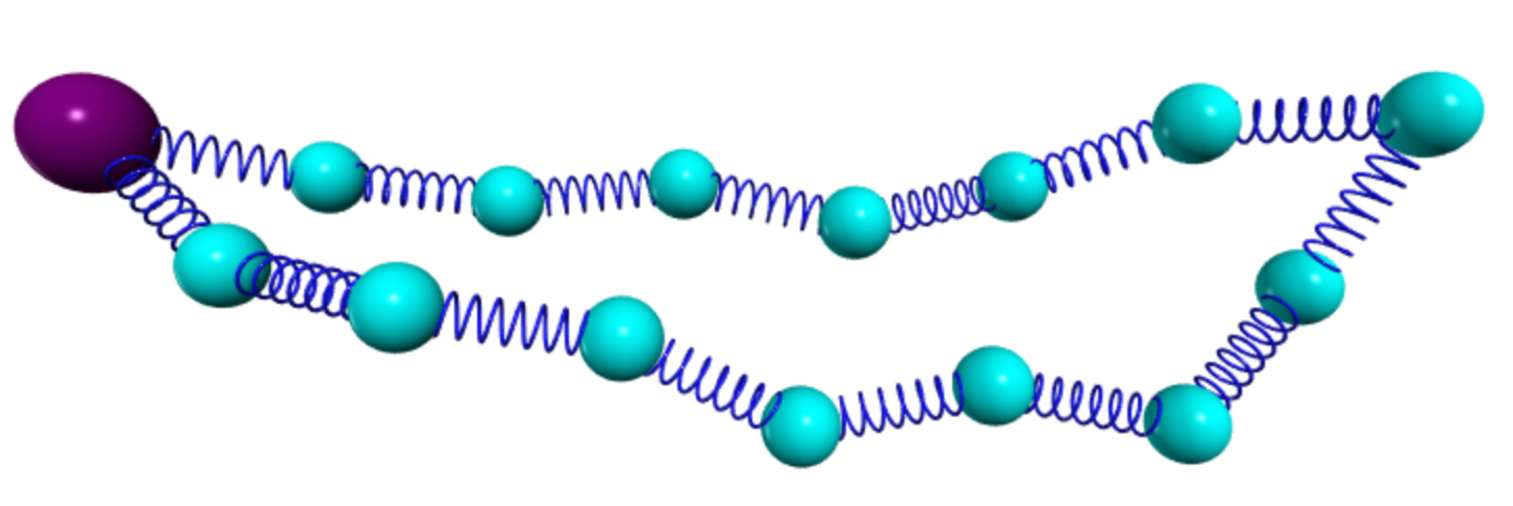
\includegraphics[width=0.8\linewidth]{beadspring}
    \caption{Sketch of the bead-spring loop model. The magenta bead represents the SPB and other cyan beads represent the chromosome segments.}
    \label{fig:beadspring}
\end{figure}

To model the chromosome in fission yeast during nuclear oscillation, we also need a looping structure like the bead-rod model above. The first bead represents the SPB, shown in Fig. \ref{fig:beadspring}. The dynamical equation is similar to the bead-rod model, can be written as following
\begin{equation}
    \label{eq:beadspringEq}
    \xi \frac{d \mathbf{r}_i}{d t} = \mathbf{F}_i^{u} + \mathbf{F}_i^{spring} + \mathbf{F}_i^{e} + \mathbf{F}_i^{b}
\end{equation}
The notations here are the same as the bead-rod model. In addition, the Brownain force, external force and the potential force are the same as in the bead-rod model. What is different is that the \emph{pseudo} force is not needed and the constraint force is replaced by the spring force $\mathbf{F}_i^{spring}$. Notice that for a bead in a loop, there are two springs connecting to it. Thus
\begin{equation}
    \label{eq:springForce}
    \mathbf{F}_i^{spring} = F_i^s(Q_i)\mathbf{u}_i - F_{i-1}^s(Q_{i-1})\mathbf{u}_{i-1}
\end{equation}
here, $F_i^s(Q_i)$ is the tension of the $i^{\rm{th}}$ spring and $Q_i$ is the length of the spring. $\mathbf{u}_i$ is the unit vector for the orientation of the $i^{\rm{th}}$ spring.

There are different type of springs we can use for the model. Here, we will introduce two most commonly used ones and both are used somewhere in the later chapters.

$\bullet$ The Hookean spring

The Hookean spring is a linear spring, where the tension of spring depends linearly on the length. 
\begin{equation}
    \label{eq:hookeanSpring}
    F^{Hookean} = H (Q-Q_0)
\end{equation}
where $H$ is the Hookean spring constant and $Q_0$ is the natural length of the spring. In practical $Q_0$ is set to $a$, which equals to the length of the bead-rod model. However, sometimes the zero length springs are used. We will point out when needed. 

$\bullet$ The Finite Extensible Nonlinear Elastic (FENE) spring

The FENE spring is another commonly used spring. The force law of the spring is
\begin{equation}
    \label{eq:feneSpring}
    F^{FENE} = \frac{H Q}{1-(Q/R_0)^2}
\end{equation}
here $R_0$ is the maximal length of the spring. As we can see in Eq. \eqref{eq:feneSpring}, $F^{FENE}\rightarrow\infty$ when $Q\rightarrow R_0$. 




%********************************** %Second Section  *************************************

\section{The Brownian Dynamics simulation method}
\label{sec:the_brownian_dynamics_simulation_method}
After introducing the model, in this section, we will illustrate how to simulation the model numerically. Since we will plan to do most of the theoretical analysis in the later chapters and the simulation results are used to benchmark, it is convenient that we show the methods of simulation before that. 

The Brownian Dynamics (BD) simulation is a kind of Molecule Dynamics (MD) simulation technique. The governing equation of each monomer or particle is integrated to get the trajectories. And physical quantities are measured by ensemble average over trajectories of thousands of monomers. In our situation, the governing equations are Eq. \eqref{eq:beadrodEq} or Eq. \eqref{eq:beadspringEq}. Our interested quantities are something like the average space distance between two beads, the typical size of the polymer and the characteristic time scale of the system dynamics. These are all tractable by BD simulations. 

In the following subsections, we will introduce the algorithms used to do the bead-rod and bead-spring simulation separately. The simulation code is implemented in C++2011. Most the simulation are computed in our clusters with $X86$ architecture.

\subsection{BD simulation of the bead-rod model}
\label{sub:bd_of_bead_rod_model}

The goal of simulation is essentially to solve the first order ordinary stochastic differential equation Eq. \eqref{eq:beadrodEq} numerically. However, the simple integration algorithm such as the Euler algorithm would not work here. This is because of the implicit constraint force $\mathbf{F}_i^{c}$. Here we employ the predictor-corrector algorithm introduced by Liu \cite{Liu1989}. 

To simplify the illustration of the algorithm, we will ignore all complex potential forces and the external force in Eq. \eqref{eq:beadrodEq}, i.e. $\mathbf{F}_i^{u} = \mathbf{F}_i^{e} = \mathbf{0}$. It is easy to add them back after knowing the algorithm. The dynamical equation after simplification looks 
\begin{equation}
    \label{eq:beadrodSimple}
    \frac{d \mathbf{r}_i}{d t} = \frac{1}{\xi}\left(\mathbf{F}_i^{c} + \mathbf{F}_i^{pseudo} + \mathbf{F}_i^{b}\right)
\end{equation}

The predictor-corrector algorithm is a two step algorithm and can be divided into the predict step and correct step. In the predict step, the next time step position is evaluated without considering the constraints
\begin{equation}
    \label{eq:beadrodPredict}
    \mathbf{r}_i^*(t+\Delta t) = \mathbf{r}_i(t) + \frac{1}{\xi}(\mathbf{F}_i^{pseudo} + \mathbf{F}_i^{b})\Delta t
\end{equation}
In order to do the calculation, we need to evaluate the Brownian force and the \emph{pseudo} force first. Here we will show how to do that one by one.

$\bullet$ Evaluation of the Brownain force $\mathbf{F}_i^{b}$


$\bullet$ Evaluation of the \emph{pseudo} force $\mathbf{F}_i^{pseudo}$


\subsection{BD simulation of the bead-spring model}
\label{sub:bd_of_bead_spring_model}

And we nondimensionalize the dynamical equation by rescaling the variable in the following way:
\begin{equation}
    \label{eq:dimensionless}
    \mathbf{r}^{\prime}\to \mathbf{r}/a;~t^{\prime}\to t/(\xi a^2/k_BT);~\mathbf{F}^{\prime}\to\mathbf{F}/(k_BT/a).
\end{equation}
After the rescaling, the length unit is set to the size of the rod. Without causing of confusing, we will ignore the prime in our notation. 



%********************************** % Third Section  *************************************
\section{The Monte-Carlo simulation of the bead-rod model}
\label{sec:the_monte_carlo_simulation_of_the_bead_rod_model}


%********************************** % Fourth Section  *************************************

\section{Summary}
\label{sec:summary}


